% Deterministically generated directly from the frozen numerical cell maps.
\begin{minipage}[t]{0.31\textwidth}\centering
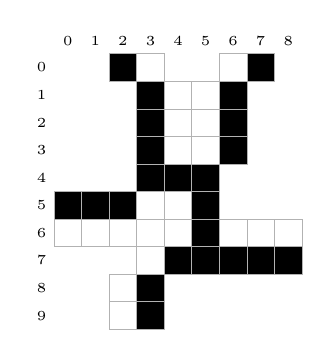
\begin{tikzpicture}[x=0.35cm,y=-0.35cm]
\filldraw[fill=black,draw=gray!60,line width=0.25pt] (0,5) rectangle ++(1,1);
\filldraw[fill=white,draw=gray!60,line width=0.25pt] (0,6) rectangle ++(1,1);
\filldraw[fill=black,draw=gray!60,line width=0.25pt] (1,5) rectangle ++(1,1);
\filldraw[fill=white,draw=gray!60,line width=0.25pt] (1,6) rectangle ++(1,1);
\filldraw[fill=black,draw=gray!60,line width=0.25pt] (2,0) rectangle ++(1,1);
\filldraw[fill=black,draw=gray!60,line width=0.25pt] (2,5) rectangle ++(1,1);
\filldraw[fill=white,draw=gray!60,line width=0.25pt] (2,6) rectangle ++(1,1);
\filldraw[fill=white,draw=gray!60,line width=0.25pt] (2,8) rectangle ++(1,1);
\filldraw[fill=white,draw=gray!60,line width=0.25pt] (2,9) rectangle ++(1,1);
\filldraw[fill=white,draw=gray!60,line width=0.25pt] (3,0) rectangle ++(1,1);
\filldraw[fill=black,draw=gray!60,line width=0.25pt] (3,1) rectangle ++(1,1);
\filldraw[fill=black,draw=gray!60,line width=0.25pt] (3,2) rectangle ++(1,1);
\filldraw[fill=black,draw=gray!60,line width=0.25pt] (3,3) rectangle ++(1,1);
\filldraw[fill=black,draw=gray!60,line width=0.25pt] (3,4) rectangle ++(1,1);
\filldraw[fill=white,draw=gray!60,line width=0.25pt] (3,5) rectangle ++(1,1);
\filldraw[fill=white,draw=gray!60,line width=0.25pt] (3,7) rectangle ++(1,1);
\filldraw[fill=black,draw=gray!60,line width=0.25pt] (3,8) rectangle ++(1,1);
\filldraw[fill=black,draw=gray!60,line width=0.25pt] (3,9) rectangle ++(1,1);
\filldraw[fill=white,draw=gray!60,line width=0.25pt] (4,1) rectangle ++(1,1);
\filldraw[fill=white,draw=gray!60,line width=0.25pt] (4,2) rectangle ++(1,1);
\filldraw[fill=white,draw=gray!60,line width=0.25pt] (4,3) rectangle ++(1,1);
\filldraw[fill=black,draw=gray!60,line width=0.25pt] (4,4) rectangle ++(1,1);
\filldraw[fill=white,draw=gray!60,line width=0.25pt] (4,5) rectangle ++(1,1);
\filldraw[fill=white,draw=gray!60,line width=0.25pt] (4,6) rectangle ++(1,1);
\filldraw[fill=black,draw=gray!60,line width=0.25pt] (4,7) rectangle ++(1,1);
\filldraw[fill=white,draw=gray!60,line width=0.25pt] (5,1) rectangle ++(1,1);
\filldraw[fill=white,draw=gray!60,line width=0.25pt] (5,2) rectangle ++(1,1);
\filldraw[fill=white,draw=gray!60,line width=0.25pt] (5,3) rectangle ++(1,1);
\filldraw[fill=black,draw=gray!60,line width=0.25pt] (5,4) rectangle ++(1,1);
\filldraw[fill=black,draw=gray!60,line width=0.25pt] (5,5) rectangle ++(1,1);
\filldraw[fill=black,draw=gray!60,line width=0.25pt] (5,6) rectangle ++(1,1);
\filldraw[fill=black,draw=gray!60,line width=0.25pt] (5,7) rectangle ++(1,1);
\filldraw[fill=white,draw=gray!60,line width=0.25pt] (6,0) rectangle ++(1,1);
\filldraw[fill=black,draw=gray!60,line width=0.25pt] (6,1) rectangle ++(1,1);
\filldraw[fill=black,draw=gray!60,line width=0.25pt] (6,2) rectangle ++(1,1);
\filldraw[fill=black,draw=gray!60,line width=0.25pt] (6,3) rectangle ++(1,1);
\filldraw[fill=white,draw=gray!60,line width=0.25pt] (6,6) rectangle ++(1,1);
\filldraw[fill=black,draw=gray!60,line width=0.25pt] (6,7) rectangle ++(1,1);
\filldraw[fill=black,draw=gray!60,line width=0.25pt] (7,0) rectangle ++(1,1);
\filldraw[fill=white,draw=gray!60,line width=0.25pt] (7,6) rectangle ++(1,1);
\filldraw[fill=black,draw=gray!60,line width=0.25pt] (7,7) rectangle ++(1,1);
\filldraw[fill=white,draw=gray!60,line width=0.25pt] (8,6) rectangle ++(1,1);
\filldraw[fill=black,draw=gray!60,line width=0.25pt] (8,7) rectangle ++(1,1);
\node[font=\tiny] at (0.5,-0.45) {0};
\node[font=\tiny] at (1.5,-0.45) {1};
\node[font=\tiny] at (2.5,-0.45) {2};
\node[font=\tiny] at (3.5,-0.45) {3};
\node[font=\tiny] at (4.5,-0.45) {4};
\node[font=\tiny] at (5.5,-0.45) {5};
\node[font=\tiny] at (6.5,-0.45) {6};
\node[font=\tiny] at (7.5,-0.45) {7};
\node[font=\tiny] at (8.5,-0.45) {8};
\node[font=\tiny] at (-.45,0.5) {0};
\node[font=\tiny] at (-.45,1.5) {1};
\node[font=\tiny] at (-.45,2.5) {2};
\node[font=\tiny] at (-.45,3.5) {3};
\node[font=\tiny] at (-.45,4.5) {4};
\node[font=\tiny] at (-.45,5.5) {5};
\node[font=\tiny] at (-.45,6.5) {6};
\node[font=\tiny] at (-.45,7.5) {7};
\node[font=\tiny] at (-.45,8.5) {8};
\node[font=\tiny] at (-.45,9.5) {9};
\end{tikzpicture}\\[4pt]\texttt{box}
\end{minipage}\hfill
\begin{minipage}[t]{0.31\textwidth}\centering
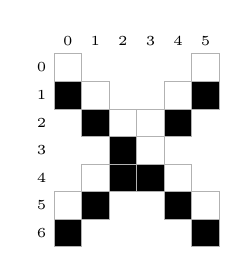
\begin{tikzpicture}[x=0.35cm,y=-0.35cm]
\filldraw[fill=white,draw=gray!60,line width=0.25pt] (0,0) rectangle ++(1,1);
\filldraw[fill=black,draw=gray!60,line width=0.25pt] (0,1) rectangle ++(1,1);
\filldraw[fill=white,draw=gray!60,line width=0.25pt] (0,5) rectangle ++(1,1);
\filldraw[fill=black,draw=gray!60,line width=0.25pt] (0,6) rectangle ++(1,1);
\filldraw[fill=white,draw=gray!60,line width=0.25pt] (1,1) rectangle ++(1,1);
\filldraw[fill=black,draw=gray!60,line width=0.25pt] (1,2) rectangle ++(1,1);
\filldraw[fill=white,draw=gray!60,line width=0.25pt] (1,4) rectangle ++(1,1);
\filldraw[fill=black,draw=gray!60,line width=0.25pt] (1,5) rectangle ++(1,1);
\filldraw[fill=white,draw=gray!60,line width=0.25pt] (2,2) rectangle ++(1,1);
\filldraw[fill=black,draw=gray!60,line width=0.25pt] (2,3) rectangle ++(1,1);
\filldraw[fill=black,draw=gray!60,line width=0.25pt] (2,4) rectangle ++(1,1);
\filldraw[fill=white,draw=gray!60,line width=0.25pt] (3,2) rectangle ++(1,1);
\filldraw[fill=white,draw=gray!60,line width=0.25pt] (3,3) rectangle ++(1,1);
\filldraw[fill=black,draw=gray!60,line width=0.25pt] (3,4) rectangle ++(1,1);
\filldraw[fill=white,draw=gray!60,line width=0.25pt] (4,1) rectangle ++(1,1);
\filldraw[fill=black,draw=gray!60,line width=0.25pt] (4,2) rectangle ++(1,1);
\filldraw[fill=white,draw=gray!60,line width=0.25pt] (4,4) rectangle ++(1,1);
\filldraw[fill=black,draw=gray!60,line width=0.25pt] (4,5) rectangle ++(1,1);
\filldraw[fill=white,draw=gray!60,line width=0.25pt] (5,0) rectangle ++(1,1);
\filldraw[fill=black,draw=gray!60,line width=0.25pt] (5,1) rectangle ++(1,1);
\filldraw[fill=white,draw=gray!60,line width=0.25pt] (5,5) rectangle ++(1,1);
\filldraw[fill=black,draw=gray!60,line width=0.25pt] (5,6) rectangle ++(1,1);
\node[font=\tiny] at (0.5,-0.45) {0};
\node[font=\tiny] at (1.5,-0.45) {1};
\node[font=\tiny] at (2.5,-0.45) {2};
\node[font=\tiny] at (3.5,-0.45) {3};
\node[font=\tiny] at (4.5,-0.45) {4};
\node[font=\tiny] at (5.5,-0.45) {5};
\node[font=\tiny] at (-.45,0.5) {0};
\node[font=\tiny] at (-.45,1.5) {1};
\node[font=\tiny] at (-.45,2.5) {2};
\node[font=\tiny] at (-.45,3.5) {3};
\node[font=\tiny] at (-.45,4.5) {4};
\node[font=\tiny] at (-.45,5.5) {5};
\node[font=\tiny] at (-.45,6.5) {6};
\end{tikzpicture}\\[4pt]\texttt{cruceA}
\end{minipage}\hfill
\begin{minipage}[t]{0.31\textwidth}\centering
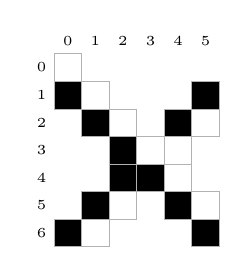
\begin{tikzpicture}[x=0.35cm,y=-0.35cm]
\filldraw[fill=white,draw=gray!60,line width=0.25pt] (0,0) rectangle ++(1,1);
\filldraw[fill=black,draw=gray!60,line width=0.25pt] (0,1) rectangle ++(1,1);
\filldraw[fill=black,draw=gray!60,line width=0.25pt] (0,6) rectangle ++(1,1);
\filldraw[fill=white,draw=gray!60,line width=0.25pt] (1,1) rectangle ++(1,1);
\filldraw[fill=black,draw=gray!60,line width=0.25pt] (1,2) rectangle ++(1,1);
\filldraw[fill=black,draw=gray!60,line width=0.25pt] (1,5) rectangle ++(1,1);
\filldraw[fill=white,draw=gray!60,line width=0.25pt] (1,6) rectangle ++(1,1);
\filldraw[fill=white,draw=gray!60,line width=0.25pt] (2,2) rectangle ++(1,1);
\filldraw[fill=black,draw=gray!60,line width=0.25pt] (2,3) rectangle ++(1,1);
\filldraw[fill=black,draw=gray!60,line width=0.25pt] (2,4) rectangle ++(1,1);
\filldraw[fill=white,draw=gray!60,line width=0.25pt] (2,5) rectangle ++(1,1);
\filldraw[fill=white,draw=gray!60,line width=0.25pt] (3,3) rectangle ++(1,1);
\filldraw[fill=black,draw=gray!60,line width=0.25pt] (3,4) rectangle ++(1,1);
\filldraw[fill=black,draw=gray!60,line width=0.25pt] (4,2) rectangle ++(1,1);
\filldraw[fill=white,draw=gray!60,line width=0.25pt] (4,3) rectangle ++(1,1);
\filldraw[fill=white,draw=gray!60,line width=0.25pt] (4,4) rectangle ++(1,1);
\filldraw[fill=black,draw=gray!60,line width=0.25pt] (4,5) rectangle ++(1,1);
\filldraw[fill=black,draw=gray!60,line width=0.25pt] (5,1) rectangle ++(1,1);
\filldraw[fill=white,draw=gray!60,line width=0.25pt] (5,2) rectangle ++(1,1);
\filldraw[fill=white,draw=gray!60,line width=0.25pt] (5,5) rectangle ++(1,1);
\filldraw[fill=black,draw=gray!60,line width=0.25pt] (5,6) rectangle ++(1,1);
\node[font=\tiny] at (0.5,-0.45) {0};
\node[font=\tiny] at (1.5,-0.45) {1};
\node[font=\tiny] at (2.5,-0.45) {2};
\node[font=\tiny] at (3.5,-0.45) {3};
\node[font=\tiny] at (4.5,-0.45) {4};
\node[font=\tiny] at (5.5,-0.45) {5};
\node[font=\tiny] at (-.45,0.5) {0};
\node[font=\tiny] at (-.45,1.5) {1};
\node[font=\tiny] at (-.45,2.5) {2};
\node[font=\tiny] at (-.45,3.5) {3};
\node[font=\tiny] at (-.45,4.5) {4};
\node[font=\tiny] at (-.45,5.5) {5};
\node[font=\tiny] at (-.45,6.5) {6};
\end{tikzpicture}\\[4pt]\texttt{cruceB}
\end{minipage}\hfill
